%BeginMC
\question
If immigration is greater than emigration and if the birth rate is greater than the death rate then

\begin{choices}
\correctchoice if nothing changes then the population will eventually reach or exceed the carrying capacity of the environment.%EndChoice
\choice the population has plenty of resources.%EndChoice
\choice the population will experience exponential growth.%EndChoice
\choice the death rate will likely decrease and the birth rate will likely increase.%EndChoice
\choice the number of predators will also increase.%EndChoice
\end{choices}
%EndMC

%BeginMC
\question
A 20-year study of gray squirrels observed that the population size decreased during the first 15 years but increased during the last five years. With only this information, which of the following is the best explanation for the observed pattern?

\begin{choices}
\correctchoice The population size at the start of the study was greater than the carrying capacity but the population size eventually fell below carrying capacity. %EndChoice
\choice The population size of squirrel predators increased during the first 15 years and decreased during the last five years. %EndChoice
\choice The effects of a severe drought caused a decrease in the amount of their normal food for 15 years but the squirrels eventually switched to a new food. %EndChoice
\choice The population was part of a trophic cascade. %EndChoice
\choice A better competitor, such as fox squirrels, prevented the gray squirrels from getting all of the food they needed to survive.%EndChoice
\end{choices}
%EndMC


%BeginMC
\question
When the number of individuals in a population remains more or less the same over time in the specific place where these individuals live, then this population has reached the \underline{\hspace{2cm}} of that place.

\begin{choices}
\choice exponential growth capacity%EndChoice
\choice maximum growth capacity%EndChoice
\choice logisitic growth capacity%EndChoice
\correctchoice carrying capacity%EndChoice
\choice population density%EndChoice
\end{choices}
%EndMC

%BeginMC
\question
The type of growth curve shown in the figure below is a

\begin{multicols}{2} 
\begin{choices}
\correctchoice logistic growth curve.%EndChoice
\choice exponential growth curve.%EndChoice
\choice carrying capacity growth curve.%EndChoice
\choice population density growth curve.%EndChoice
\choice maximum growth curve.%EndChoice
\end{choices}
\columnbreak
	\hfill 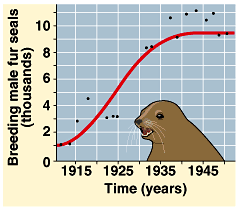
\includegraphics[width=5cm]{img/logistic_growth.png}
\end{multicols}
%EndMC

%BeginMC
\question
Assuming a population has unlimited resources, exponential growth occurs because

\begin{choices}
\correctchoice the birth rate exceeds the death rate.%EndChoice
\choice the emigration rate exceeds the death rate.%EndChoice
\choice the death rate exceeds the birth rate.%EndChoice
\choice the immigration rate equals the death rate and the emigration rate equals the birth rate.%EndChoice
\choice the emigration exceeds the birth rate.%EndChoice
\end{choices}
%EndMC





%BeginMC
\question
Consider the food chain grass $\to$ grasshopper $\to$ mouse $\to$ snake $\to$ hawk. How much of the chemical energy fixed by photosynthesis of the grass (100\%) is available to the hawk?

\begin{choices}
\correctchoice 0.01\%%EndChoice
\choice 0.1\%%EndChoice
\choice 1\%%EndChoice
\choice 10\%%EndChoice
\choice 60\%%EndChoice
\end{choices}
%EndMC
%BeginMC
\question
Bobcats eat forest mice. The mice eat seeds. Suppose a fire on the forest floor reduces the amount of seeds by 75\%.  Before the fire, the population of mice sustained a bobcat population of 8. What will \emph{most likely} happen to the bobcat population as a result of the fire? The bobcat population will

\begin{choices}
\correctchoice decrease to two after a delay. %EndChoice
\choice decrease to two almost immediately. %EndChoice
\choice decrease by two but most will survive. %EndChoice
\choice increase as the bobcats shift to another food source. %EndChoice
\choice not be affected because the mice survived the fire. %EndChoice
\end{choices}
%EndMC


%BeginMC
\question
Some fish, like the goby in the picture below, live inside sponges. Sponges are a type of living organism. The goby benefits from the shelter provided by the sponge. The sponge receives no apparent benefit. As described here, this is an example of

\begin{multicols}{2} 
\begin{choices}
\correctchoice commensalism.%EndChoice
\choice predation.%EndChoice
\choice mutualism.%EndChoice
\choice parasitism.%EndChoice
\choice symbiosis.%EndChoice
\end{choices}
\columnbreak
	\hfill 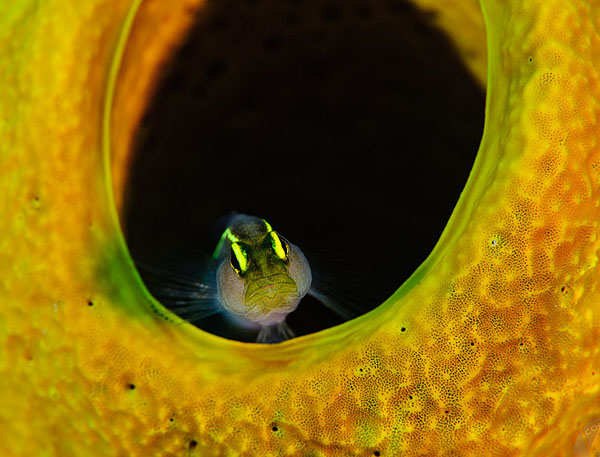
\includegraphics[width=4cm]{img/goby_sponge.jpg}
\end{multicols}
%EndMC

%BeginMC
\question
The ``role'' or ``job'' of a species in a community, represented by all of the resources needed by the species, is called 

\begin{choices}
\correctchoice the niche.%EndChoice
\choice the resource.%EndChoice
\choice a predator.%EndChoice
\choice a predator or prey.%EndChoice
\choice a producer or consumer.%EndChoice
\end{choices}
%EndMC






%BeginMC
\question
If humans stopped fishing along the coast of Alaska, what will probably happen to the kelp forest and why?

\begin{choices}
\correctchoice The kelp abundance will increase because the sea urchin abundance will probably decrease.%EndChoice
\choice The kelp abundance will remain about the same. The kelp are not part of this community, so the kelp would not be affected.%EndChoice
\choice The kelp abundance will decrease because more fish will be present to eat the kelp.%EndChoice
\choice The kelp abundance will decrease. Sea otters eat urchins and urchins eat kelp. Because there were fewer otters to eat urchins, the number of urchins increased. The urchins therefore ate more kelp so the kelp abundance decreased.%EndChoice
\choice The kelp abundance will increase because of the symbiotic relationship between kelp and fishes. Fishes are necessary for kelp to reproduce.%EndChoice
\end{choices}
%EndMC

%BeginMC
\question
The southeastern region of Missouri lies within the temperate broadleaf forest ecosystem. According to the climograph below, the temperate broadleaf forest

\begin{multicols}{2} 
\begin{choices}
\choice never has more than about 220 cm (87 inches) of rainfall per year.%EndChoice
\correctchoice has an average of 60--220 cm of precipitation per year.%EndChoice
\choice has more rain and similar temperatures to the northern coniferous forest.%EndChoice
\choice always has more precipitation than the temperate grassland.%EndChoice
\choice is never warmer than the temperate grassland.%EndChoice
\end{choices}
\columnbreak
	\hfill 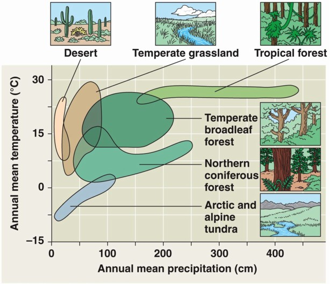
\includegraphics[width=6cm]{img/climograph.png}
\end{multicols}
%EndMC

%BeginMC
\question
In summer 2012, the Midwest experienced one of the worst droughts in recorded history. Which of the following statements is the best prediction of how this drought will have affected the Gulf of Mexico dead zone during summer 2012?

\begin{choices}
\correctchoice The dead zone will be smaller because the Mississippi River will carry less water so fewer nutrients will be carried to the Gulf of Mexico.%EndChoice
\choice The dead zone will be smaller because farmers, anticipating the drought, would not have added fertilizer to the crop fields the spring before the drought.%EndChoice
\choice The dead zone will be similar to previous years because the drought is not likely to affect the amount of water that flows out through the Mississippi River.%EndChoice
\choice The dead zone will be larger because the reduced volume of water will concentrate the nutrients that enter the Gulf of Mexico.%EndChoice
\choice The dead zone will be smaller because less freshwater will enter the Gulf of Mexico, allowing more saltwater fishes to live around the mouth of the river.%EndChoice
\end{choices}
%EndMC

%BeginMC
\question
The dead zone in the Gulf of Mexico and other oceans around the globe occurs when

\begin{choices}
\choice an excess of nutrients causes an algal bloom. The algae consume all of the oyxgen in the water for photosynthesis, so other organisms can no longer live there.%EndChoice
\choice eutrophication causes an absence of nutrients in the zone.%EndChoice
\choice commercial fishers overharvest shrimp, crab, fishes and other sea animals.%EndChoice
\correctchoice an excess of nutrients causes an algal bloom, followed by death of the algae. Decomposition of the algae uses up the oxygen in the water, so other organisms can no longer live there.%EndChoice
\choice global climate change causes the water to become too warm to sustain life.%EndChoice
\end{choices}
%EndMC

%BeginMC
\question
Which of the following statements about symbiotic relationships is true?

\begin{choices}
\correctchoice A relationship that appears to be commensalism may in fact be mutualistism or parasitism.%EndChoice
\choice Both organisms are harmed in a parasitic relationship.%EndChoice
\choice Both symbiotic organisms usually benefit from the relationship.%EndChoice
\choice The most efficient type of parasite is one that kills its host.%EndChoice
\choice Neither organism benefits in a symbiotic relationship.%EndChoice
\end{choices}
%EndMC

%BeginMC
\question
On average, the amount of primary consumer biomass is about \underline{\hspace{2cm}} less than the amount of primary producer biomass.

\begin{choices}
\choice 10\%%EndChoice
\choice 20\%%EndChoice
\choice 50\%%EndChoice
\choice 80\%%EndChoice
\correctchoice 90\%%EndChoice
\end{choices}
%EndMC

%BeginMC
\question
Considering your knowledge of the dead zone and the causes of microscopic algae blooms, the Gulf of Mexico ecosystem is emph{most likely} to be limited by which of the following nutrients?

\begin{choices}
\choice carbon%EndChoice
\choice \ce{CO2}%EndChoice
\choice hydrogen%EndChoice
\choice oxygen%EndChoice
\correctchoice nitrogen%EndChoice
\end{choices}
%EndMC

%BeginMC
\question
Plants produce water vapor during photosynthesis, which goes from the plant to the atmosphere. The water vapor in the atmosphere eventually falls back to the earth as rain. This process would be part of

\begin{choices}
\correctchoice the water cycle.%EndChoice
\choice energy flow.%EndChoice
\choice plant metabolism.%EndChoice
\choice the entire ecosystem.%EndChoice
\choice the energy cycle.%EndChoice
\end{choices}
%EndMC


%BeginMC
\question
Species Old can nest anywhere in a certain kind of pine tree. Recently, due to global climate change, Species New has arrived from down south. Species New also nests in the same kind of pine tree. However, Species New can only nest in the outermost 50\% of any branch (shown in darker color).  Species Old chases away Species New in the inner part of the tree but ignores Species New in the outer part of the tree. What will \emph{most likely} happen in the tree after a few years?

\begin{multicols}{2} 
\begin{choices}
\correctchoice Species New will nest in the outer part of the tree and Species Old will nest in the inner part of the tree.%EndChoice
\choice Species Old will prevent Species New from making nests so Species New will die out in this location.%EndChoice
\choice Species New will prevent Species Old from making nests so Species Old will die out in this location.%EndChoice
\choice Both species will nest in the outer part of the tree in equal numbers but only Species Old will nest in the inner part of the tree.%EndChoice
\choice Species Old will nest more often in the outer part of the tree.%EndChoice
\choice Neither species will survive because they can't nest in the entire tree. %EndChoice
\end{choices}
\columnbreak
	\hfill \includegraphics[width=5cm]{ex3_partition_tree.png}
\end{multicols}
%EndMC

%BeginMC
\question
Higher elevations on a mountain experience less precipitation and cooler temperatures than low elevations.  As you descended from the top of the mountain, you would notice a change in the types of plants and animals present in the community.  This is analogous to the changes in the ecosystems if you walked 

\begin{choices}
\correctchoice from the north pole to the equator.%EndChoice
\choice east to west over different altitudes.%EndChoice
\choice west to east at one latitude.%EndChoice
\choice from the equator to the south pole.%EndChoice
\choice from the north pole to the south pole.%EndChoice
\end{choices}
%EndMC


%BeginMC
\question
According to the figure below, which is most correct about the offspring produced by Type I organisms?

\begin{multicols}{2}
\begin{choices}
\choice Most offspring will die at a very young age.%EndChoice
\correctchoice Most offspring will live most of their natural lifespan.%EndChoice
\choice About the same number of offspring will die every year.%EndChoice
\choice About 50\% of the individuals will die every year.%EndChoice
\choice Most offspring will die about half way through their natural life.%EndChoice
\end{choices}
\columnbreak
	\hfill 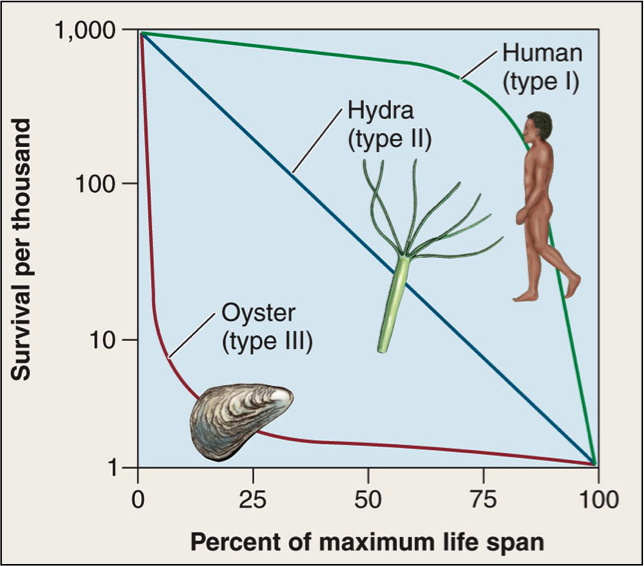
\includegraphics[width=6cm]{img/survivorship.png}
\end{multicols}
%EndMC

%BeginMC
\question
The land on the south side of the Himalayan mountain range (below) receives relatively high levels of rainfall and has fertile farmlands.  The land north of the mountain range is hot and dry and can't be farmed.  Which of the following is true.

\begin{multicols}{2}
\begin{choices}
\choice The south side of the Himalayan mountain range is in a rain shadow.%EndChoice
\choice The desert in southern China warms the north side of the mountain range, causing it to dry out.%EndChoice
\choice The cool, moist Indian Ocean air heats up as it rises, releasing its precipitation as it passes the tops of the mountains, and this warm, now dry air cools as it descends on the leeward side of the range.%EndChoice
\correctchoice Warm, moist air from the Indian Ocean blows north, rises and cools, releasing precipitation as it moves up the south side of the range, and this cool, now dry air mass heats up as it descends on the north side of the range.%EndChoice
\choice The warm, moist air is too dense to rise over the height of Mount Everest and the other mountains in this range so the moisture remains on the south side of the range.%EndChoice
\end{choices}
\columnbreak
	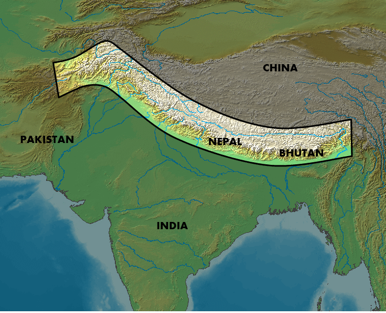
\includegraphics[width=8cm]{img/himalayas.png}
\end{multicols}
%EndMC

%BeginMC
\question
The Mediterranean coast and coastal California have similar types of ecosystems. This is because

\begin{choices}
\correctchoice they have similar climates.%EndChoice
\choice they have similar types of organisms.%EndChoice
\choice they are both wine-growing regions.%EndChoice
\choice they have similar types of communities.%EndChoice
\choice they are at similar latitudes.%EndChoice
\end{choices}
%EndMC


%BeginMC
\question
The difference between emigration and immigration is

\begin{choices}
\correctchoice emigration is when individuals move out of a population; immigration is when individuals move into a population.%EndChoice
\choice the direction in which individuals are moving into or out of the population.%EndChoice
\choice emigration is when individuals move into a population; immigration is when individuals move out of a population.%EndChoice
\choice the overall movement of individuals among populations.%EndChoice
\choice emigration is when individuals move out of a population; immigration is when individuals move out of a community.%EndChoice
\end{choices}
%EndMC

%BeginMC
\question
Which of the following are important biotic (living) factors that can affect the  organization of communities?

\begin{choices}
\choice precipitation, wind%EndChoice
\choice nutrient availability, soil pH%EndChoice
\correctchoice predation, competition%EndChoice
\choice temperature, water%EndChoice
\choice light intensity, seasonality%EndChoice
\end{choices}
%EndMC

%BeginMC
\question
Based on this food web, which letter represents an organism that is a primary producer? The arrows point in the direction of energy flow (to higher trophic levels).

\begin{multicols}{2} 
\begin{choices}
\choice A%EndChoice
\correctchoice B%EndChoice
\choice C%EndChoice
\choice D%EndChoice
\choice E%EndChoice
\end{choices}
\columnbreak
	\hfill 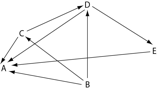
\includegraphics{img/foodweb.png}
\end{multicols}
%EndMC

%BeginMC
\question
Carrying capacity

\begin{choices}
\choice is seldom reached by most population because the environment has plenty of resources.%EndChoice
\correctchoice is the maximum population size that a particular environment can support.%EndChoice
\choice does not for most species most of the time.%EndChoice
\choice is determined by birth and death rates, and emigration and immigration rates.%EndChoice
\choice describes the stress a population undergoes due to limited resources.%EndChoice
\end{choices}
%EndMC

%BeginMC
\question
Which of the following is \textit{not} one of the four factors that play a role in population growth rate?

\begin{choices}
\choice Immigration.%EndChoice
\choice Death rate.%EndChoice
\choice Emigration.%EndChoice
\choice Birth rate.%EndChoice
\correctchoice Demography.%EndChoice
\end{choices}
%EndMC

%BeginMC
\question
A transient killer whale eats seals. The seals ate fish. The fish ate part of a dead killer whale laying on the sea floor, but also ate smaller live squid. You do not know what the squid might have eaten. The fish in this example is acting as \underline{\hspace{2cm}}. (Choose the best answer)

\begin{choices}
\correctchoice a consumer and a decomposer.%EndChoice
\choice a secondary consumer and a primary consumer.%EndChoice
\choice a secondary consumer and a decomposer.%EndChoice
\choice a secondary consumer, a decomposer, and a consumer one trophic level higher than the killer whale.%EndChoice
\choice a consumer and a producer.%EndChoice
\end{choices}
%EndMC

%BeginMC
\question
After transient orca began to prey on sea otters, what happened to the kelp forest?

\begin{choices}
\choice The kelp abundance remained about the same. The kelp are not part of this community, so the kelp could not be affected.%EndChoice
\choice The kelp abundance remained about the same. Only the predator-prey interactions between Orca and otters were important, so nothing happened to the kelp.%EndChoice
\choice The kelp abundance increased. Otters dislodge kelp with their playful antics.  Because there were fewer otters, less kelp was dislodged so the kelp abundance increased.%EndChoice
\correctchoice The kelp abundance decreased. Sea otters eat urchins and urchins eat kelp.  Because there were fewer otters to eat urchins, the number of urchins increased.  The urchins therefore ate more kelp so the kelp abundance decreased.%EndChoice
\choice The kelp abundance decreased. Sea otters and kelp have a symbiotic relationship. Without the sea otters, the symbiotic relationship was broken and so the kelp abundance decreased.%EndChoice
\end{choices}
%EndMC

%BeginMC
\question
Competition occurs between two different species in a community when

\begin{choices}
\correctchoice both species need the same resources that is in limited supply.%EndChoice
\choice both species are searching for mates.%EndChoice
\choice one species is a predator of the other.%EndChoice
\choice both species have partitioned resources.%EndChoice
\choice one species is a parasite of the other.%EndChoice
\end{choices}
%EndMC

